\documentclass[13pt]{beamer}
\usetheme{Frankfurt}
\usecolortheme{beaver}

\usepackage[spanish]{babel}
\usepackage{amsmath}
\usepackage{amsfonts}
\usepackage{amssymb}
\usepackage{color}
\usepackage{xcolor}
\usepackage{listings}
\usepackage{graphicx}
\usepackage{wrapfig}

\definecolor{codegreen}{rgb}{0,0.6,0}
\definecolor{codegray}{rgb}{0.5,0.5,0.5}
\definecolor{codepurple}{rgb}{0.58,0,0.82}
\definecolor{backcolour}{rgb}{0.95,0.95,0.92}

\lstdefinestyle{mystyle}{
    basicstyle=\tiny,
    commentstyle=\color{codegreen},
    keywordstyle=\color{magenta},
    numberstyle=\tiny\color{codegray},
    stringstyle=\color{codepurple},
    basicstyle=\ttfamily\footnotesize,
    breakatwhitespace=false,         
    breaklines=true,                 
    captionpos=b,                    
    keepspaces=true,                 
    numbers=left,                    
    numbersep=5pt,                  
    showspaces=false,                
    showstringspaces=false,
    showtabs=false,                  
    tabsize=2,
	xleftmargin=8pt
}

\lstset{literate=
	{á}{{\'a}}1 {é}{{\'e}}1 {í}{{\'i}}1 {ó}{{\'o}}1 {ú}{{\'u}}1
	{Á}{{\'A}}1 {É}{{\'E}}1 {Í}{{\'I}}1 {Ó}{{\'O}}1 {Ú}{{\'U}}1
	{à}{{\`a}}1 {è}{{\`e}}1 {ì}{{\`i}}1 {ò}{{\`o}}1 {ù}{{\`u}}1
	{À}{{\`A}}1 {È}{{\'E}}1 {Ì}{{\`I}}1 {Ò}{{\`O}}1 {Ù}{{\`U}}1
	{ä}{{\"a}}1 {ë}{{\"e}}1 {ï}{{\"i}}1 {ö}{{\"o}}1 {ü}{{\"u}}1
	{Ä}{{\"A}}1 {Ë}{{\"E}}1 {Ï}{{\"I}}1 {Ö}{{\"O}}1 {Ü}{{\"U}}1
	{â}{{\^a}}1 {ê}{{\^e}}1 {î}{{\^i}}1 {ô}{{\^o}}1 {û}{{\^u}}1
	{Â}{{\^A}}1 {Ê}{{\^E}}1 {Î}{{\^I}}1 {Ô}{{\^O}}1 {Û}{{\^U}}1
	{ã}{{\~a}}1 {ẽ}{{\~e}}1 {ĩ}{{\~i}}1 {õ}{{\~o}}1 {ũ}{{\~u}}1
	{Ã}{{\~A}}1 {Ẽ}{{\~E}}1 {Ĩ}{{\~I}}1 {Õ}{{\~O}}1 {Ũ}{{\~U}}1
	{œ}{{\oe}}1 {Œ}{{\OE}}1 {æ}{{\ae}}1 {Æ}{{\AE}}1 {ß}{{\ss}}1
	{ű}{{\H{u}}}1 {Ű}{{\H{U}}}1 {ő}{{\H{o}}}1 {Ő}{{\H{O}}}1
	{ç}{{\c c}}1 {Ç}{{\c C}}1 {ø}{{\o}}1 {å}{{\r a}}1 {Å}{{\r A}}1
	{€}{{\euro}}1 {£}{{\pounds}}1 {«}{{\guillemotleft}}1
	{»}{{\guillemotright}}1 {ñ}{{\~n}}1 {Ñ}{{\~N}}1 {¿}{{?`}}1 {¡}{{!`}}1 
}

\lstset{style=mystyle, basicstyle=\scriptsize}

\author{Shao Jie Hu Chen \and Mario Megías Mateo \and Jesús Samuel García Carballo}
\title{Práctica 2. Divide y Vencerás}
\subtitle{Algorítmica}
%\logo{
\includegraphics[scale=0.05]{logo-ugr.jpeg}}
\institute{Equipo Rojo}
%\date{}
%\subject{}
%\setbeamercovered{transparent}
\setbeamertemplate{navigation symbols}{}

\begin{document}
	
	\begin{frame}[plain]
		\maketitle
		% \begin{center}
		% 	
\includegraphics[scale=0.15]{logo-ugr.jpeg}
		% \end{center}
	\end{frame}
	
	\begin{frame}
		\frametitle{Índice de contenidos}
		\tableofcontents
	\end{frame}

    % Introducción

    \section{Introducción}

    \begin{frame}
        \frametitle{Objetivos y motivación}

        \begin{itemize}
            \item \textbf{Implementar} algoritmo de tipo Divide y Vencerás.
            \item \textbf{Saber reconocer} el alcance y las limitaciones de algoritmos 
            de tipo Divide y Vencerás en ejemplos particulares.
        \end{itemize}

    \end{frame}

    \begin{frame}
        \frametitle{Metodología}

        \begin{figure}[h]
            \centering
            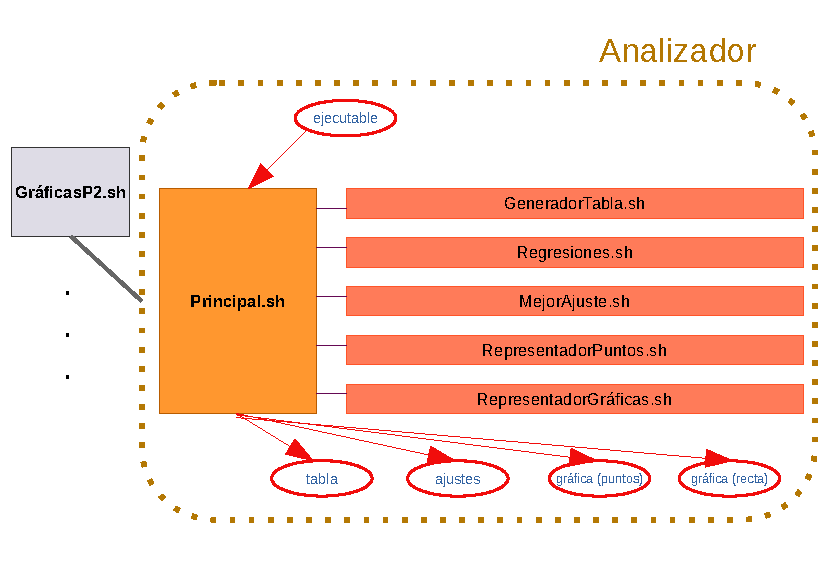
\includegraphics[scale=0.65]{img/esquema_graphkiller.pdf}
            \caption{Esquema de funcionamiento del \textbf{Analizador} \cite{Rojo2022}. Elaboración propia.}
            \label{fig:analizador}
        \end{figure}
    \end{frame}

    \begin{frame}
        \frametitle{Equipo empleado}

        \begin{block}{Especificaciones técnicas del equipo}
            \begin{itemize}
                \item \textbf{Procesador}: Intel(R) Core(TM) i7-9750H CPU @ 2.60GHz
                \item \textbf{Memoria RAM:} 32 GB DDR4
                \item \textbf{Sistema Operativo}: Ubuntu 20.04.4 LTS
            \end{itemize}
        \end{block}
    \end{frame}


    % Ejercicio 1

    \section{Ejercicio 1: Vectores no repetidos}

    \begin{frame}
        \frametitle{Lemas claves}
            \begin{block}{Lema de la cota superior}
                \label{lem:1}
                Sea i con $0 \leqslant i < n$ fijo, tal que $v[i]=i+k$, con $k \in \mathbb N$. 
                Entonces $v[j] \neq j$, $\forall j \in \mathbb N$ con $i < j < n$. 
            \end{block}
            \begin{block}{Lema de la cota inferior}
                \label{lem:2}
                Sea i con $0 < i < n$ fijo, tal que $v[i]=i-k$ con 
                $k \in \mathbb N$. Entonces $v[j] \neq j$,  $\forall j$ con $0 \leqslant j < i$. 
            \end{block}
    \end{frame}

	 \begin{frame}
		\frametitle{Caso obvio. Pseudocódigo.}
		\lstinputlisting[caption=Pseudocódigo asociado al caso obvio., label={alg:1a-obvio}]{listing/ejer1a-pseudo-obvio.txt}
	\end{frame}

	 \begin{frame}
		\frametitle{Caso obvio. Implementación en C++.}
		\lstinputlisting[language=C++, firstline=93, lastline=106, caption=Implementación en C++ 
		del algoritmo basado en la búsqueda lineal., label={cod:1a-obvio}]{../src/ejercicio-1-comp-fija-no-repetidos.cpp} 
	\end{frame}

	\begin{frame}
		\frametitle{Análisis de eficiencia caso obvio.}
		 
		 \begin{block}{Eficiencia Teórica}
		 	$$T(n) \in \mathcal{O}(n)$$
		 \end{block}
	 
	\end{frame}

	\begin{frame}
		\frametitle{Análisis de eficiencia caso obvio.}
	\end{frame}

	\begin{frame}
		\frametitle{Caso Divide y Vencerás. Pseudocódigo.}
		\lstinputlisting[caption=Pseudocódigo asociado al caso Divide y Vencerás., label={alg:1a-dyv}]{listing/ejer1a-pseudo-dyv.txt}
	\end{frame}

	\begin{frame}
		\frametitle{Caso Divide y Vencerás. Implementación.}
		\lstinputlisting[language=C++, firstline=119, lastline=131, 
		caption=Implementación en C++ del algoritmo basado en Divide y Vencerás., label={cod:1a-dyv}]
		{../src/ejercicio-1-comp-fija-no-repetidos.cpp} 
	\end{frame}

	\begin{frame}
		\frametitle{Caso Divide y Vencerás. Determinación del umbral.}
		% Aquí viene la imagen
	\end{frame}

	\begin{frame}
	\frametitle{Caso Divide y Vencerás. Análisis de eficiencia.}
			\begin{equation}
				T(n) = \left\{ \begin{array}{lr} T(n/2) + c & \text{si } n > \text{UMBRAL}\\ n & \text{si } n \leqslant \text{UMBRAL} \end{array} \right.
				\label{eq:1a-efi-dyv-rec}
			\end{equation}
			\begin{equation}
			T(n) = c_{1} + c_{2} \log_2(n) \implies \boxed{T(n) \in O(\log_2(n))}
			\label{eq:1a-eficiencia-lineal}
			\end{equation}
	\end{frame}

    \section{Ejercicio 1: Vectores repetidos}

    \begin{frame}
        \frametitle{Descripción}
        \begin{block}{Problema}
            Dado un vector de n componentes ordenado de menor a mayor (con \textbf{valores repetidos}), 
            encontrar $i$ tal que $v[i] = i$. 
        \end{block}

        \begin{alertblock}{Fallo del algoritmo anterior}
            El algoritmo propuesto para el caso con valores no repetidos \textbf{no es válido}.
        \end{alertblock}
    \end{frame}

    \begin{frame}
        \frametitle{Ejemplo de funcionamiento erróneo}
        \begin{figure}
            \centering
            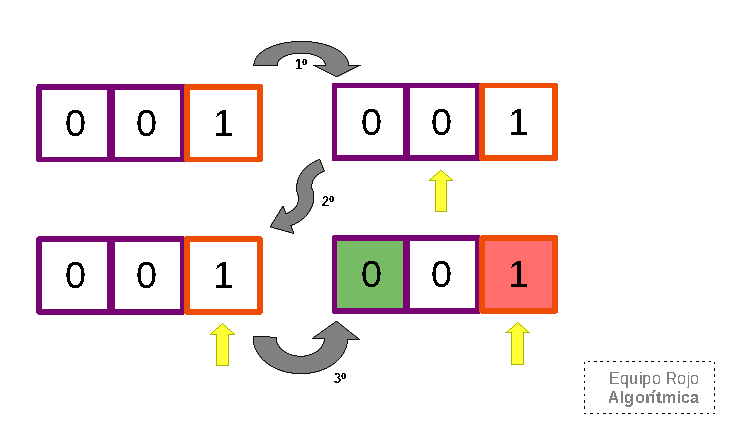
\includegraphics[scale=0.81]{img/esquema_fallo1a.pdf}
            \caption{Vector con elementos repetidos para el que falla 
            el algoritmo anterior. Elaboración propia.}
            \label{fig:fallo-1a}
        \end{figure}
    \end{frame}

    \begin{frame}
        \frametitle{Modificación del algoritmo}

        \lstinputlisting[caption=Pseudocódigo asociado al caso Divide y Vencerás., label={alg:1b-dyv}]{listing/ejer1b-pseudo-dyv.txt}
    \end{frame}

    \begin{frame}
        \begin{exampleblock}{Implementación en C++}
            \lstinputlisting[language=C++, firstline=114, lastline=134, label={cod:1b-dyv}]
            {../src/ejercicio-1-comp-fija-repetidos.cpp} 
        \end{exampleblock}
    \end{frame}

    \begin{frame}
        \frametitle{Análisis de Eficiencia Teórica}

        \begin{block}{Ecuación en diferencias asociada}
            \begin{equation}
                T(n) = \left\{ \begin{array}{lr} 2 T(n/2) + c & \text{si } n > \text{UMBRAL}\\ n & \text{si } n \leqslant \text{UMBRAL} \end{array} \right.
                \label{eq:1b-efi-dyv-rec}
            \end{equation}
        \end{block}

        Por tanto:

        \begin{alertblock}{Orden de eficiencia del algoritmo}
            \begin{equation*}
                \boxed{T(n) \in O(n)}
            \end{equation*}
        \end{alertblock}
        
    \end{frame}

    \begin{frame}
        \frametitle{Resultados empíricos}

        \begin{columns}
            \begin{column}{0.2\textwidth}
                \begin{table}
                    \tiny
                    \centering
                    \begin{tabular}{|r|r|}
                        \hline
                        $N$ & $T(ms)$ \\
                        \hline
                        1 & 0.0017 \\ 
                        250000 & 1.2638 \\ 
                        500000 & 2.5020 \\ 
                        750000 & 3.8801 \\ 
                        1000000 & 4.7835 \\ 
                        1250000 & 5.6027 \\ 
                        1500000 & 7.8714 \\ 
                        1750000 & 9.1403 \\ 
                        2000000 & 9.6127 \\ 
                        2250000 & 10.3977 \\ 
                        2500000 & 10.8430 \\ 
                        2750000 & 12.5853 \\ 
                        3000000 & 15.4864 \\ 
                        3250000 & 17.7592 \\ 
                        3500000 & 18.3230 \\ 
                        3750000 & 18.6021 \\ 
                        4000000 & 19.0520 \\ 
                        4250000 & 19.8521 \\ 
                        4500000 & 20.6940 \\ 
                        4750000 & 20.9706 \\ 
                        \hline
                    \end{tabular}
                \end{table}
            \end{column}

            \begin{column}{0.2\textwidth}
                \begin{table}
                    \tiny
                    \centering
                    \begin{tabular}{|r|r|}
                        \hline
                        $N$ & $T(ms)$ \\
                        \hline

                        5000000 & 21.6910 \\ 
                        5250000 & 22.3115 \\ 
                        5500000 & 25.4420 \\ 
                        5750000 & 27.9453 \\ 
                        6000000 & 30.8848 \\ 
                        6250000 & 33.7447 \\ 
                        6500000 & 34.7666 \\ 
                        6750000 & 35.5849 \\ 
                        7000000 & 35.9877 \\ 
                        7250000 & 37.1252 \\ 
                        7500000 & 37.9441 \\ 
                        7750000 & 38.4063 \\ 
                        8000000 & 38.9629 \\ 
                        8250000 & 39.6185 \\ 
                        8500000 & 40.0429 \\ 
                        8750000 & 41.1611 \\ 
                        9000000 & 41.9953 \\ 
                        9250000 & 42.0843 \\ 
                        9500000 & 42.5158 \\ 
                        9750000 & 42.8710 \\ 

                        \hline
                    \end{tabular}
                \end{table}
            \end{column}

            \begin{column}{0.6\textwidth}
                \begin{figure}
                    \centering
                    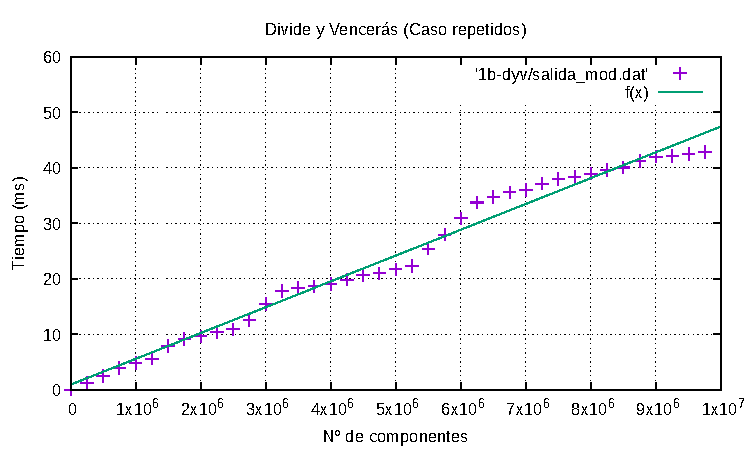
\includegraphics[scale=0.5]{img/e1b-dyv}
                    % \caption{Gráfica de tiempos de ejecución para el caso Divide y Vencerás, 
                    % con f(x) y coeficiente de regresión especificada por \ref{eq:1b-dyv-eficiencia}.}
                    % \label{fig:1b-dyv-graph}
                \end{figure}

                \footnotesize

                \begin{equation*}
                    \boxed{f(x) = 4,6553 \cdot 10^{-6} x + 0.8657, R^2 = 0,9834}
                    \label{eq:1b-dyv-eficiencia}
                \end{equation*}
            \end{column}
        \end{columns}
    \end{frame}

    % \begin{frame}
    %     \frametitle{Eficiencia híbrida}
    %     \begin{figure}
    %         \centering
    %         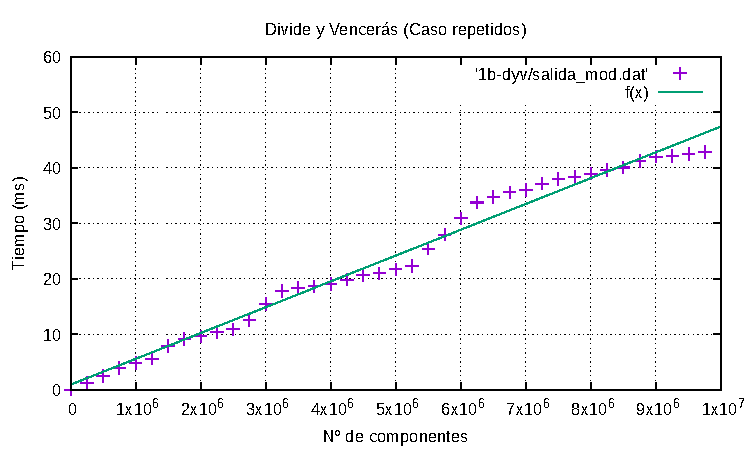
\includegraphics[scale=0.8]{img/e1b-dyv}
    %         % \caption{Gráfica de tiempos de ejecución para el caso Divide y Vencerás, 
    %         % con f(x) y coeficiente de regresión especificada por \ref{eq:1b-dyv-eficiencia}.}
    %         % \label{fig:1b-dyv-graph}
    %     \end{figure}

    %     \begin{equation*}
    %         \boxed{f(x) = 4,6553 \cdot 10^{-6} x + 0.8657, R^2 = 0,9834}
    %         \label{eq:1b-dyv-eficiencia}
    %     \end{equation*}
    % \end{frame}

    % \begin{frame}
    %     \frametitle{Comparación con el caso obvio}

    %     \begin{figure}
    %         \centering
    %         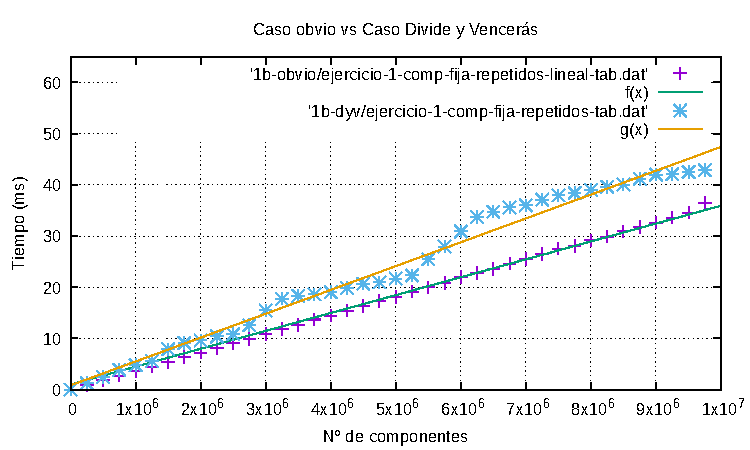
\includegraphics[scale=0.66]{img/e1b-comp.pdf}
    %         % \caption{Gráfica de comparación tiempos de ejecución para Divide y Vencerás y caso obvio.}
    %         \label{fig:1b-comp}
    %     \end{figure}

    %     \begin{alertblock}{¡Atención!}
    %         Los tiempos de ejecución del algoritmo tipo Divide y Vencerás son \textbf{peores que el obvio}. 
    %     \end{alertblock}
    % \end{frame}

    % \begin{frame}
    %     \frametitle{Posible explicación: Sobrecarga de la pila}
    %     \begin{itemize}
    %         \item En los vectores generados, la distribución 
    %         general es la aparición del índice
    %         buscado en los elementos finales del vector.
    %         \item Ambos casos analizan casi todo el vector.
    %         \item El algoritmo Divide y Vencerás \textbf{introduce información de contexto
    %         en la pila} por cada llamada recursiva, lo que penaliza el rendimiento global del
    %         algoritmo. 
    %     \end{itemize}
    % \end{frame}

    % Ejercicio 2

    \section{Ejercicio 2: Unificación de vectores}


    \subsection{Caso obvio}

	\begin{frame}
		\frametitle{Caso Obvio. Implementación en C++.}
		\lstinputlisting[language=C++, firstline=118, lastline=130, 
		caption=Implementación en C++ del algoritmo obvio., label={cod:1a-dyv}]
		{../src/ejercicio-2-mezcla.cpp} 
	\end{frame}

    \begin{frame}
		\frametitle{Análisis de eficiencia caso obvio.}
		 
		 \begin{block}{Eficiencia Teórica}
		 	$$T(n) \in \mathcal{O}(nk^{2})$$
	    \end{block}
	 
	\end{frame}

    \begin{frame}
        \frametitle{Eficiencia empírica: Caso k fijo.}

        \begin{figure}
            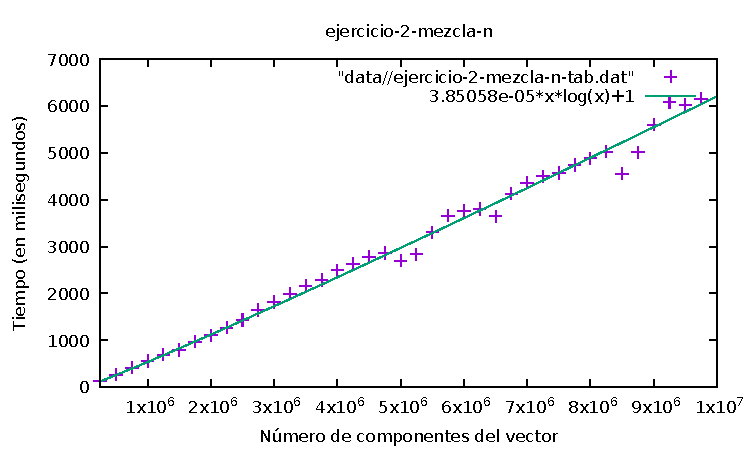
\includegraphics[width=0.7\textwidth]{../data/2-obvio/ejercicio-2-mezcla-n-graph.pdf}
            \caption{Gráfica de tiempos de ejecución (en $\mu$s) con respecto a los elementos del vector para el caso obvio.}
        \end{figure}
    \end{frame}

    \begin{frame}
        \frametitle{Eficiencia empírica: Caso n fijo.}

        \begin{figure}
            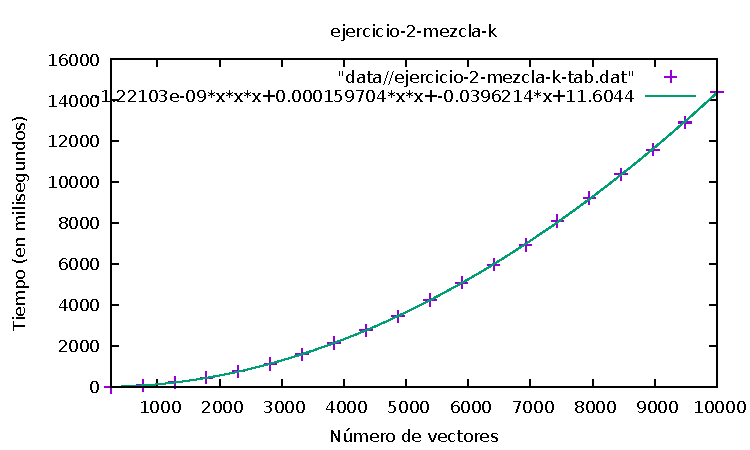
\includegraphics[width=0.7\textwidth]{../data/2-obvio/ejercicio-2-mezcla-k-graph.pdf}
            \caption{Gráfica de tiempos de ejecución (en $\mu$s) respecto al número de vectores para el caso obvio.}
        \end{figure}
    \end{frame}

    \begin{frame}
		\frametitle{Caso Divide y Vencerás. Implementación en C++.}
		\lstinputlisting[language=C++, firstline=120, lastline=149, 
		caption=Implementación en C++ del algoritmo divide y vencerás., label={cod:1a-dyv}]
		{../src/ejercicio-2-mezcla-dyv.cpp} 
	\end{frame}

    \subsection{Caso divide y vencerás}

    \begin{frame}
		\frametitle{Análisis de eficiencia caso divide y vencerás.}
		 \begin{block}{Eficiencia Teórica}
		 	$$T(n) \in \mathcal{O}(nk^{2})$$
		 \end{block}
	 
	\end{frame}


    \begin{frame}
        \frametitle{Eficiencia empírica: Caso k fijo.}

        \begin{figure}
            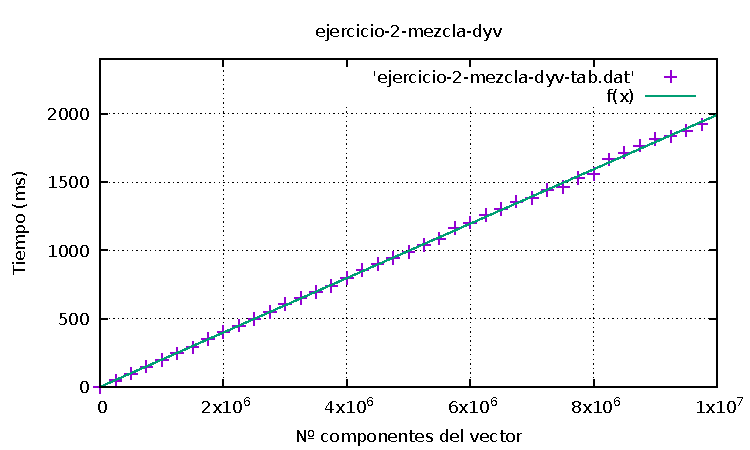
\includegraphics[width=0.7\textwidth]{../data/2-dyv/ejercicio-2-mezcla-dyv-graph.pdf}
            \caption{Gráfica de tiempos de ejecución (en $\mu$s) con respecto a los elementos del vector para el caso divide y vencerás.}
        \end{figure}
    \end{frame}

    \begin{frame}
        \frametitle{Eficiencia empírica: Caso n fijo.}

        \begin{figure}
            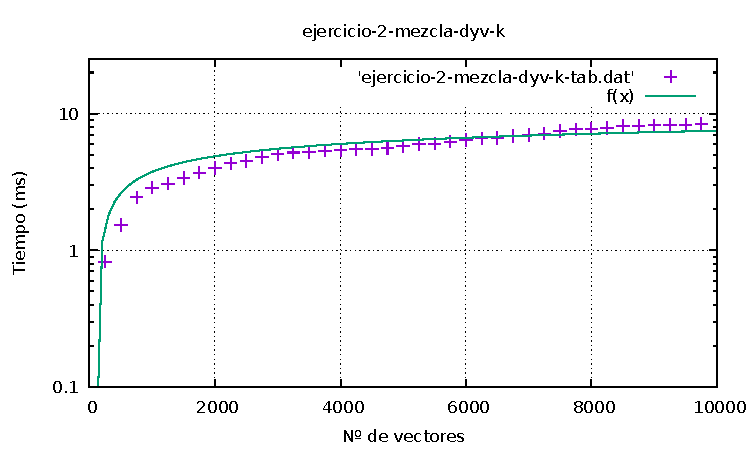
\includegraphics[width=0.7\textwidth]{../data/2-dyv/ejercicio-2-mezcla-dyv-k-graph.pdf}
            \caption{Gráfica de tiempos de ejecución (en $\mu$s) respecto al número de vectores para el caso divide y vencerás.}
        \end{figure}
    \end{frame}

    \begin{frame}
        \frametitle{Comparación con el caso obvio}

        \begin{figure}
            \centering
            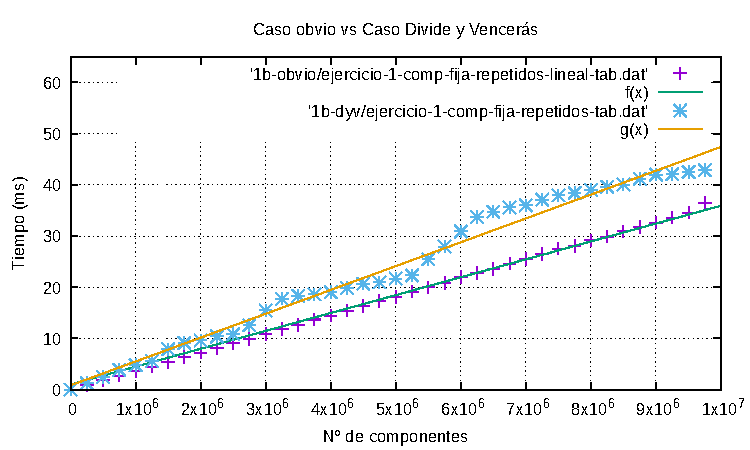
\includegraphics[scale=0.66]{img/e1b-comp.pdf}
            % \caption{Gráfica de comparación tiempos de ejecución para Divide y Vencerás y caso obvio.}
            \label{fig:1b-comp}
        \end{figure}

    \end{frame}

    % Conclusiones

    % Bibliografía

    \section{Bibliografía}

    \begin{frame}
        \begin{thebibliography}{0}
            \bibitem{Verdegay2017} Verdegay Galdeano. (2017). Lecciones de Algorítmica / José Luis Verdegay. Técnica Avicam.
            \bibitem{Cormen2017} Cormen. (2017). Introduction to algorithms / Thomas H. Cormen... [et al.] (3rd ed.). PHI Learning.
            \bibitem{Garrido2018} Garrido Carrillo. (2018). Estructuras de datos avanzadas: con soluciones en C++ / A. Garrido. Universidad de Granada.        
            \bibitem{Rojo2022} Hu Chen. (2022). Práctica 1: Análisis de Eficiencia de Algoritmos / Shao Jie Hu, J. Samuel García y Mario Megías.      
        \end{thebibliography}
    \end{frame}

\end{document}